
%%%%%%%%%%%%%%%%%%%%%%%%%%%%%%%%%%%%%%%%%%%%%%%%%%%%%%%%%%%%%%%%%%%%%%%%
%    INSTITUTE OF PHYSICS PUBLISHING                                   %
%                                                                      %
%   `Preparing an article for publication in an Institute of Physics   %
%    Publishing journal using LaTeX'                                   %
%                                                                      %
%    LaTeX source code `ioplau2e.tex' used to generate `author         %
%    guidelines', the documentation explaining and demonstrating use   %
%    of the Institute of Physics Publishing LaTeX preprint files       %
%    `iopart.cls, iopart12.clo and iopart10.clo'.                      %
%                                                                      %
%    `ioplau2e.tex' itself uses LaTeX with `iopart.cls'                %
%                                                                      %
%%%%%%%%%%%%%%%%%%%%%%%%%%%%%%%%%%
%
%
% First we have a character check
%
% ! exclamation mark    " double quote  
% # hash                ` opening quote (grave)
% & ampersand           ' closing quote (acute)
% $ dollar              % percent       
% ( open parenthesis    ) close paren.  
% - hyphen              = equals sign
% | vertical bar        ~ tilde         
% @ at sign             _ underscore
% { open curly brace    } close curly   
% [ open square         ] close square bracket
% + plus sign           ; semi-colon    
% * asterisk            : colon
% < open angle bracket  > close angle   
% , comma               . full stop
% ? question mark       / forward slash 
% \ backslash           ^ circumflex
%
% ABCDEFGHIJKLMNOPQRSTUVWXYZ 
% abcdefghijklmnopqrstuvwxyz 
% 1234567890
%
%%%%%%%%%%%%%%%%%%%%%%%%%%%%%%%%%%%%%%%%%%%%%%%%%%%%%%%%%%%%%%%%%%%
%
%%novalidate

\documentclass[11pt,a4paper,final]{iopart}
\newcommand{\gguide}{{\it Preparing graphics for IOP journals}}
%Uncomment next line if AMS fonts required
\usepackage{iopams}  
\usepackage{graphicx}
\usepackage[breaklinks=true,colorlinks=true,linkcolor=blue,urlcolor=blue,citecolor=blue]{hyperref}
\usepackage[english]{babel}
\usepackage{siunitx}
\usepackage{graphicx}
\usepackage{amsfonts,amssymb,amstext,amsthm,verbatim,times,cancel,epsfig} 
\usepackage{fancyhdr}
\usepackage{setspace}
\usepackage[italian]{varioref}
\usepackage{verbatim}
\usepackage{caption}
\usepackage[utf8]{inputenc}
\usepackage{wrapfig}

\usepackage{booktabs}
\usepackage[toc,page]{appendix}

\begin{document}

\title[]{\vspace{-3.5cm}\\A method for detecting gravitational wave signals from an ensemble of known pulsars}

\author{M. Buono$^{1,2}$, R. De Rosa$^{1,2}$, L. D'Onofrio$^{1,2}$, L. Errico$^{1,2}$, C. Palomba$^{3}$, O. Piccinni$^{3,4}$, V. Sequino$^{1,2}$}
\address{$^1$Università di Napoli “Federico II”, I-80126 Napoli, Italy
\\$^2$INFN, Sezione di Napoli, I-80126 Napoli, Italy
\\$^3$INFN, Sezione di Roma, I-00185 Roma, Italy
\\$^4$Università di Roma “La Sapienza",I-00185 Roma, Italy}


\begin{abstract}
This work describes a new method to improve detection efficiency for continuous gravitational waves combining information from known pulsars that could not be identified individually. “Known” indicates objects like the Crab or Vela pulsar, whose position, rotational frequency and its evolution are known with high accuracy. 
We propose a new statistic of ensemble $t$ combining statistics from individual pulsar, defined through 5-vec method.
Using a collection of Band Sample-Data files of O2 run for LIGO detectors, we apply the proposed method to software injections in order to reconstruct and analyze the distributions of $t$. We also study the performance of our method using the inferred distributions of $t$ and increasing the number of injected pulsars with different “strengths” of injected amplitudes. Using a set of real pulsars, we found no evidence of CW signals in O2 data using analysis of ensemble.

\end{abstract}


\section{Introduction}
Gravitational wave astronomy began on September 14, 2015 when LIGO Hanford and LIGO Livingston observatories detected the first gravitational wave signal GW150914 \cite{firstdet} produced by the merger of two black holes. GW150914 demonstrated the existence of binary stellar-mass black hole systems and was also the first observation of binary black hole merger \cite{astimpl}. The first confirmed multi-messenger counterpart to a gravitational wave observation came instead with GW170817 \cite{firstBBS}. GW170817 originated  from  a  binary  neutron  star coalescence  which  was accompanied by detections across the electromagnetic spectrum.
\\So far detected signals come from coalescences of compact objects and are transient signals, confined in a short time window. Continuous gravitational waves (CWs) are a different class of signals, potentially observable by the LIGO and Virgo detectors.
\\ Isolated spinning neutron stars with non axi-symmetric mass distribution are possible sources of CWs. The gravitational signal from this type of astrophysical sources is periodic and the frequency of the signal is linked to the rotational frequency of the source.  If the neutron star is a pulsar, accurate ephemeris may be available from electromagnetic observations. Hence matched filtering techniques can be employed using waveform templates that cover the entire observing period. 
\\Recently, the LIGO-Virgo collaboration presented a search \cite{result} for gravitational waves from 222 pulsars with rotational frequencies above 10 Hz using advanced LIGO data from its first and second observing runs. This search found no evidence for gravitational-wave emission from any pulsar at either frequency. For only 22 pulsars the obtained results gave limits lower than the theoretical spin-down limit.
\\In this context, this work tries to improve detection efficiency for CWs combining information from weak sources, such as known pulsars, that could not be identified individually. 
\\“Known” indicates objects like the Crab or Vela pulsar, whose position, rotational frequency and its evolution are known with high accuracy. This search, that is a targeted search, assumes that the gravitational frequency is exactly twice the rotational frequency of the star. Methods to detect gravitational waves from an ensemble of known pulsars have already been presented by Fan, Chen and Messenger, combining F-statistic values from individual pulsar \cite{Fstat2}, and by Pitkin, Fan and Messenger, using the Hierarchical Bayesian method \cite{bayes}. 
\\In this paper, we define a new statistic $t$ for ensemble that is a particular combination of the statistics of single pulsar, defined through 5-vec method \cite{2010}.
\\This paper is organized as follows. In Sec.\ref{due}, we provide a brief background on the CW signal and the 5-vec method. In Sec.\ref{tre}, we set theoretical limits for the statistic of single pulsar and ensemble. In Sec.\ref{4}, we introduce approximated expressions for the statistics using real data and different ensemble. To reduce the computational cost of the analysis, we use a new data framework, the Band-Sampled Data (BSD) collection \cite{2019}.  In Sec.\ref{cinque},  we test the performance of our method considering different sets of injected pulsars varying the dimension of the ensemble and the "strength" of single pulsar signal. In Sec.\ref{6}, we use coherence to organize real pulsars and we apply our method to O2 data. Conclusions are presented in Sec.\ref{end}.

%\\In this paper, we define a new statistic $t$ for ensemble that is a particular combination of the statistics of single pulsar, defined through 5-vec method \cite{2010}.
% Using real data and different ensamble of pulsar, we introduce approximated expressions for the statistics in Section \ref{4}.To reduce the computational cost of the analisys, we use a new data framework, the Band-Sampled Data (BSD) collection \cite{2019}, based on the construction of BSD file, that is a band-limited, down-sampled complex time series. We test the performance of our method considering different sets of injected pulsars varying the dimension of the ensamble and the "strength" of single pulsar signal. 

\section{The gravitational wave signal}\label{due}
The CW signal emitted by a triaxial neutron star rotating at frequency $f_{rot}$ around a principal axis of inertia can be written at the detector as \cite{JKS}:
\begin{equation}\label{signal}
h(t)= \frac{1}{2}h_0 (1+\cos^2 \iota) \cos\Phi(t) F_+(t) + h_0 \cos \iota \sin \Phi(t) F_\times(t)
\end{equation}where  $F_+(t)$ and $F_\times(t)$ are the two  beam-pattern  functions, $\iota$ is the angle between the star rotation axis and the line of sight and
\begin{equation}\label{amplitude}
h_0=\frac{16\pi^2 G}{c^4} \frac{I\epsilon f_{rot}^2}{d}
\end{equation} is the gravitational wave amplitude.$\,I$ is the star moment of inertia with respect to the rotation axis, $\epsilon$ the equatorial ellipticity and $d$  the distance from the Earth. 
\\$\Phi(t)$, in  (\ref{signal}), defines the gravitational wave phase evolution inferred from pulsar radio (or X-ray) pulsations.
\\Expression in (\ref{signal}) can be described in a different way by a polarization ellipse characterized by $\eta$, the ratio of its semiminor to its semimajor axis, and by the angle $\psi$ that defines the direction of the ellipse semi-major axis respect to the celestial parallel of the source (measured counterclockwise). $\eta$ varies in the range $[-1,1]$ ($\eta=0$ for a linearly polarized wave and $\eta=\pm1$ for a circularly polarized wave) and is linked to $\iota$ by the following relation:\begin{equation}
\eta=-\frac{2\cos \iota}{1+\cos^2 \iota}\,.
\end{equation} 
The complex form of (\ref{signal}) can be expressed as:\begin{equation}
h(t)=H_0(H_+ A_+ + H_\times A_\times)e^{i\Phi(t)} \,,
\end{equation}where\begin{equation}
H_+=\frac{\cos(2\psi)-i\eta \sin(2\psi)}{\sqrt{1+\eta^2}} \qquad    H_\times=\frac{\sin(2\psi)+i\eta \cos(2\psi)}{\sqrt{1+\eta^2}}
\end{equation}
\begin{equation}\label{corramp}
 H_0=h_0 \sqrt{\frac{1+6\cos^2\iota + \cos^4 \iota}{4}}\,.
\end{equation}
The expressions of $A_+$ and $A_\times$, whose complete formulations can be found in \cite{2010}, depend on the  two  beam-pattern  functions and on the Earth sidereal angular frequency $\Omega_\oplus$. This dependence on $\Omega_\oplus$ is at the bottom of the 5-vec method, that we used in this work. 
\\After correcting for the Earth-induced Doppler effect, various relativistic effects and the source spin-down using heterodyne demodulation \cite{2019}, the signal at the detector becomes monochromatic apart from an amplitude and phase sidereal modulation:\begin{equation}
h(t)=H_0(H_+ A_+ + H_\times A_\times)e^{i(\omega_0 t + \gamma)}\,.
\end{equation}This expression is the product of a fast periodic term, with frequency $f_{gw}=\omega_0/2\pi=2f_{rot}$ and phase $\gamma$, and a slow term given by a linear combination of sines and cosines with arguments $\Omega_\oplus$ and $2\Omega_\oplus$ \cite{2010}.\\  Then, the signal at the detector is completely described by its Fourier components at the five angular frequencies $\omega_0, \omega_0\pm\Omega_\oplus ,\omega_0\pm2\Omega_\oplus$.
This set of five complex numbers constitutes the signal 5-vector,
\begin{equation}\label{5vec}
 \textbf{X} =\int_{T_{obs}}x(t) e^{-i\textbf{k} \Omega_\oplus t} e^{-i\omega_0t}dt \qquad \text{with} \qquad \textbf{k}=(0,\pm 1,\pm 2)\,.
\end{equation}
The 5-vec method consists of two matched filters in the frequency domain among the data 5-vector, $\textbf{X}$, and the signal template 5-vectors $\textbf{A}_+, \textbf{A}_\times$: \begin{equation}\label{estim}
\hat{H}_+=\frac{\textbf{X}\cdot \textbf{A}^+}{|\textbf{A}^+|^2} \qquad \text{and} \qquad \hat{H}_\times=\frac{\textbf{X}\cdot \textbf{A}^\times}{|\textbf{A}^\times|^2}\,.
\end{equation} $\textbf{A}_+$ and  $\textbf{A}_\times$ are obtained applying the definition (\ref{5vec}) by replacing the time series $x(t)$ with the two functions $A_+$ and $A_\times$. The signal template 5-vectors depend exclusively on known parameters (source position, detector position and sidereal response of the detector).
\\Assuming Gaussian noise with zero mean value, it can be shown \cite{2010} that the two quantities in (\ref{estim}) are respectively estimators of $H_0e^{i\gamma}H_+$ and $H_0e^{i\gamma}H_\times$ and that can be used to estimate the unknown parameters ($H_0$, $\psi$, $\eta$).

\section{Single pulsar and ensemble statistics}\label{tre}
The detection statistic for single pulsar can be chosen as the linear combination of the modulus of the two complex estimators in (\ref{estim}):\begin{equation}\label{thstat}
S=c_+ |\hat{H}_+|^2 +c_\times |\hat{H}_\times|^2\equiv c_+ S_+ + c_\times S_\times \,.
\end{equation}
Assuming Gaussian noise with zero mean value and variance $\sigma^2$, we study the coefficients $c_+$ and $c_\times$ optimizing the critical ratio ($\textrm{CR}$) defined as:
\begin{equation}\label{CRS}
\textrm{CR}=\frac{(\mu_{sig}-\mu_{n})^2}{\Theta^2_{n}}
\end{equation} where $\mu_{sig}$ is the mean of $S$ when a signal is present into data while $\mu_{n}$ and $\Theta_{n}$ are respectively the mean and variance of $S$ when there is noise only.
\\Maximizing the $\textrm{CR}$ respect to the two coefficients, the resulting equations are not independent (see \ref{appendix:calcoli}). There is a straight line in the plane $(c_+,c_\times)$ where the function $\textrm{CR}$ has maximum value. 
%This line is identified by the equation:
%\begin{equation}\label{der}
%c_+=\beta_+k_+\frac{c_\times}{\beta_\times k_\times}=|H_+|^2|\textbf{A}_+|^4\frac{c_\times}{|H_\times|^2|\textbf{A}_\times|^4}
%\end{equation}
A possible choice that satisfies this condition is:
\begin{equation}\label{chosN}
\bar{c}_+=|H_+|^2|\textbf{A}_+|^4 \qquad \text{and} \qquad \bar{c}_\times=|H_\times|^2|\textbf{A}_\times|^4
\end{equation}
To construct a detection statistic for an ensemble of pulsars, we introduce the following general expression:
\begin{equation}\label{tstat}
t=\sum_{i=1}^{N_s} a_i S_i
\end{equation}where $N_s$ is the number of considered pulsars and $S_i$ is the single statistic with coefficients in (\ref{chosN}). 
%\begin{equation}
%S_i=b_{+,i}S_{+,i} + b_{\times,i}S_{\times,i} \qquad \text{with} \qquad b_{+,i}\equiv c_+ \qquad b_{\times,i}\equiv c_\times
%\end{equation}
As in the previous case, it is possible to infer the theoretically best choice for the coefficient $a_i$ of the statistic of ensemble $t$, considering the $\textrm{CR}$ 
\begin{equation}\label{CRt}
\textrm{CR}= \frac{\left[\sum_{j=1}^{N_s} a_j (\mu_{sig,j}-\mu_{n,j})\right]^2}{\sum_{i=1}^{N_s} a_i^2 \Theta^2_{n,i}} \equiv \frac{\left[\sum_{j=1}^{N_s} a_j \lambda_j\right]^2}{\sum_{i=1}^{N_s} a_i^2 \Theta_{n,i}^{\,2}}
\end{equation}
%where
%\begin{equation}
%\lambda_j\equiv (\mu_{sig,j}-\mu_{n,j})^2  \qquad \text{and} \qquad \sigma_j^{\,2}\equiv \sigma^2_{n,j}
%\end{equation}
%We chose the coefficient $a_j$ maximazing the $SNR$ as a function of the $N_s$ coefficients:
%\begin{equation}
%\frac{\partial (SNR)}{\partial a_k}=\frac{2\lambda_k\left(\sum_{j=1}^{N_s}a_j \lambda_j\right)}{\sum_{i=1}^{N_s}a_i^2\sigma^2_i}-\frac{2a_k \sigma_k^2\left(\sum_{j=1}^{N_s}a_j \lambda_j\right)^2}{\left(\sum_{i=1}^{N_s}a_i^2\sigma^2_i\right)^2}=0
%\end{equation}for $k=1,..,N_s$.
%The $N_s$ equations are not independent.
Maximizing the $\textrm{CR}$ as a function of the coefficients, there is an hyperplane where the function $\textrm{CR}(a_1,..,a_{N_s})$ has maximum value.
%, identified by the equation:
%\begin{equation}
%a_k=\frac{\lambda_k}{\sigma_k^2}\frac{\left(\sum_{i=1,i\neq k}^{N_s}a_i^2\sigma^2_i\right)}{\left(\sum_{j=1,j\neq k}^{N_s}a_j \lambda_j\right)}
%\end{equation}
A particular, simple choice of the coefficients that maximizes the $\textrm{CR}$, is:
\begin{equation}\label{coeffens}
\bar{a}_k=\frac{\lambda_k}{\Theta_{n,k}^{\,2}}=\frac{H_{0,k}^2}{\sigma^4_{k}\cdot T_{obs}^2 }
\end{equation}
%\begin{equation}\label{coeffens}
%a_k=\frac{\lambda_k}{\sigma_k^{\,2}}=\frac{H_{0,k}^2(|H_{+,k}|^4|\textbf{A}_{+,k}|^4 + |H_{\times,k}|^4|\textbf{A}_{\times,k}|^4)}{\sigma^4_{x,k} (|H_{+,k}|^4|\textbf{A}_{+,k}|^4 + |H_{\times,k}|^4|\textbf{A}_{\times,k}|^4)}=\frac{H_{0,k}^2}{\sigma^4_{x,k} }
%\end{equation}
 We will indicate by $\bar{S}$ and $\bar{t}$, the statistic of single pulsar and of ensemble with coefficients respectively in (\ref{chosN}) and (\ref{coeffens}).
\\For real pulsar, $\bar{c}_+,\bar{c}_\times$ and $\bar{a}_k$ are theoretical coefficients that maximizes the CR but related to unknown quantities. Indeed, $|H_{+,\times}|^2$ depend on the unknown gravitational wave parameters $\psi$, $\eta$ and the amplitude $H_0$ is also unknown.
\\For this reason, we need approximated expressions for the coefficients in (\ref{chosN}) and (\ref{coeffens}). 

\section{Approximated expressions for $\bar{S}$ and $\bar{t}$ coefficients}\label{4}
To compare different values for the coefficients, it is important to reconstruct the statistic distributions and to analyze the Receiver Operating Characteristics (ROC) curves. ROC curves for  $\bar{S}$ and $\bar{t}$ are theoretical limits that we want to approach with an appropriate choice for the coefficients.
\\We can reconstruct statistic distributions using software injections of simulated pulsars. For each pulsar, we need to fix $\eta$, $\psi$  and the injected amplitude $H$, defined as:
\begin{equation}\label{injamp}
H=\alpha \cdot h_{min}
\end{equation} with $0<\alpha<1$. In this way, no pulsars can be detected individually since injected amplitudes are below the minimum detectable strain $h_{min}$.  For targeted search $h_{min}$ is \cite{jjj}:
\begin{equation}
\label{hminimo}
h_{min}\approx 11 \sqrt{\frac{S(f_{gw})}{T_{obs}}} 
\end{equation}
 where $S(f_{gw})$ is the one-sided power spectral density at the expected frequency $f_{gw}$.
\\The signal distribution can be built from the data itself considering a range of off-source frequencies close but different from the one where the signal is expected \cite{2014}. In these off-source frequencies, we injected a signal with the same amplitude and the same source parameters of the selected one. Since software injections provide the expected Doppler and Einstein delay and the spin-down frequency variation to the signal, it is necessary to make the appropriate corrections for each simulation (that is for each injection). 
Instead, in the case of noise, it suffices to evaluate the statistic at the selected off-source frequencies without signal injections.
\\The software injections are performed using a collection of Band-Sample Data (BSD) files \cite{2019} covering 8 months (from 4 January 2017 until the end of O2 run) of LIGO Livingston detector (LLO) and 10 Hz frequency band. 
%containing the signal of the analyzed pulsar. In this frequency band, we must check that the noise distribution is Gaussian with zero mean value and variance $\sigma$ for all the O2 run. This is an important point: using the value of $\sigma$ inferred by the distribution of the real part of the BSD reduced-analytic signal in any $1$ Hz frequency band, it is possibile to infer the theoretical noise distribution for the detection statistic.
\begin{figure}
\centering
        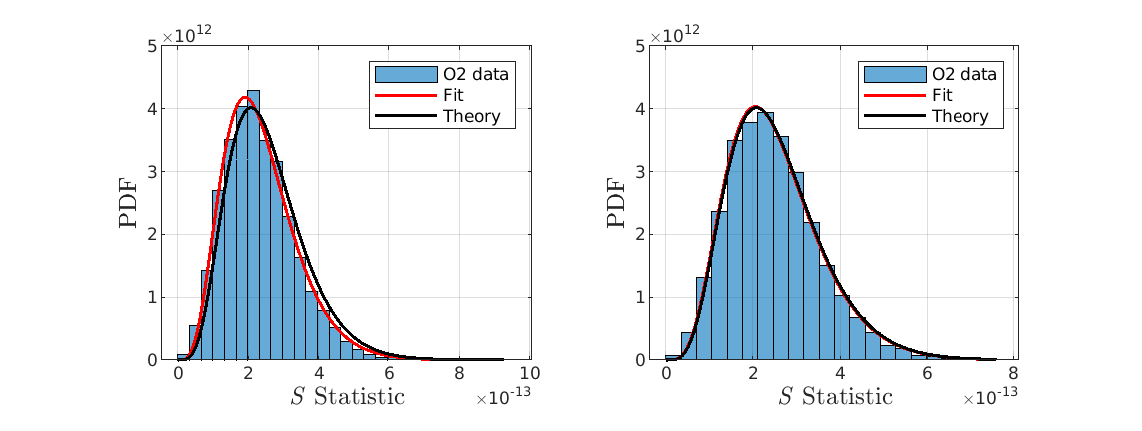
\includegraphics[clip,trim=45 0 10 0,scale=0.9]{spindown.eps}
    \caption{Experimental signal distribution (blue histogram) for the statistic of single pulsar with  $c_{+/\times}=|\textbf{A}_{+/\times}|^4$ varying the injected spin-down value ($\dot{f}_{gw}=-7\cdot10^{-9} Hz/s$ for the left plot, $\dot{f}_{gw}=-7\cdot10^{-11} Hz/s$ for the right plot) and leaving other parameters unchanged. Red line is the Gamma fit to experimental distibution while black line is the proposed Gamma distribution.} 
    \label{spindown}
    \vspace{-10pt}
\end{figure} 
\\To consider ROC curves, we need to reconstruct the distribution of $S$ in presence of signals for simulated pulsar. For the analized combinations\footnote{The analyzed combinations are $c_{+/\times}=1/2$;\, $c_{+/\times}=|\textbf{A}_{+/\times}|^4$;\, $c_{+/\times}=|\textbf{A}_{+/\times}|^2$.} of $c_+$ and $c_\times$, the signal distribution  is the weighted sum of non central $\chi^2$ random variables and in general, there is no simple analytical expression for this distribution.
\\We found empirically that Gamma distribution  can fit the experimental distribution to a good approximation for all the analyzed combinations of $c_+$ and $c_\times$. The shape and scale parameter of this Gamma distribution are inferred from mean and variance of $S$ that are known for simulated pulsar.
\\ This approximation does not depend on fixed parameters (source parameters, $\eta$, $\psi$) and on injected amplitude $H$. We noticed that the approximation gets worse increasing the spin-down value $\dot{f}_{gw}$ and leaving other parameters unchanged (Figure \ref{spindown}). In any case, high spin down values ($\sim (-10^{-9}) Hz/s$) are not usual for real pulsars.
%\\The inferred Gamma distribution is used to estimate ROC curves in a general case without needing to inject signals on real data.
\\For the statistic of single pulsar $S$, in accordance with \cite{2010}, the analysis of the ROC curves with different combinations of $c_+$ and $c_\times$ confirms that the best choice is:\begin{equation}
c_+=|\textbf{A}_+|^4 \qquad \text{and} \qquad c_\times=|\textbf{A}_\times|^4
\end{equation}  
%For example with $c_{+/\times}=|\textbf{A}_{+/\times}|^4$, there is no simple analytical expression for the signal distribution since $S$ is the weighted sum of non central $\chi^2$ random variables \cite{2014}. 
%On the other hand, by choosing $c_{+,\times}=|\textbf{A}_{+/\times}|^2$, the signal distribution is a non central $\chi^2$ distribution \cite{2010}. 
%\\In general, the distribution of the weighted sum of non central $\chi^2$ random variables has no simple expression.
For the statistic of ensemble $t$, we analyzed different choices for the coefficients $a_i$ in equation (\ref{tstat}) that takes into account the sensitivity of the detector $a_i=S^{-1}(f_{gw,i})\cdot T_{obs}^{-1}$, the squared sensitivity $ a_i=S^{-2}(f_{gw,i})\cdot T_{obs}^{-1}$, both the sensitivity and the sidereal response of the detector  $a_i=(|\textbf{A}_{+,i}|^2+|\textbf{A}_{\times,i}|^2)^2 \cdot S^{-2}(f_{gw,i})\cdot T_{obs}^{-1}$.
%\begin{itemize}
 %\item    sensitivity of the detector: $a_i=\frac{1}{S(f_{gw,i})}\equiv \frac{1}{\sigma_i^2}$;
%\item    squared sensitivity: $a_i=\frac{1}{S(f_{gw,i})^2}\equiv \frac{1}{\sigma_i^4}$;
% \item    sensitivity and sidereal response of the detector: $a_i=\frac{(|\textbf{A}_{+,i}|^2+|\textbf{A}_{\times,i}|^2)^2}{\sigma^2_{i}}$
 %\item  With frequency and distance $a_i=\frac{f_{gw}^4}{d^2 \sigma^4_{i}\cdot T_{obs}^2}$
%\end{itemize}
\\For the signal distribution of $t$, it is reasonable that the Gamma approximation works also for all the selected combination of $a_i$ (see Figure \ref{tABCD} for a particular case).
\\According to Figure \ref{choicet}, the best choice for the coefficients, that entails ROC curve closest to $\bar{t}$ ROC curve, is:
\begin{equation} \label{statt}
a_i=\frac{1}{S(f_{gw,i})\cdot T_{obs}}
\end{equation}  We have analyzed many differents sets of simulated pulsars varying the injected amplitudes and obtaining in all cases the same result.

\begin{figure}
\centering
        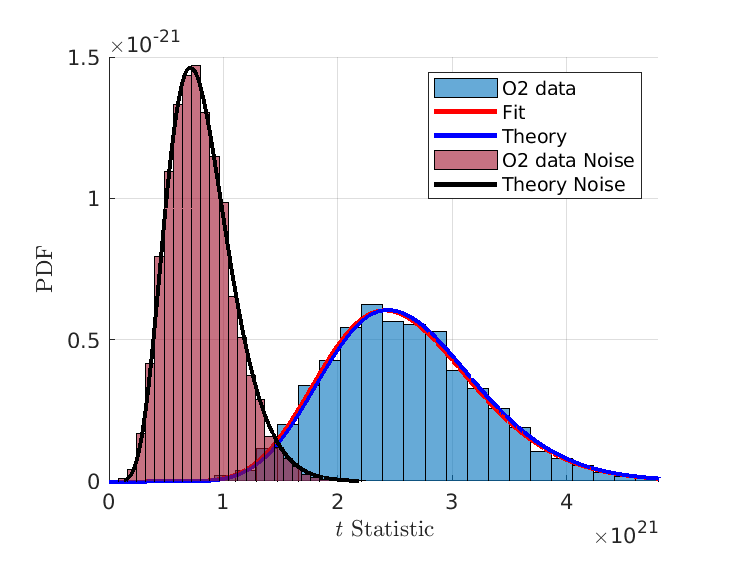
\includegraphics[scale=0.8]{ABCD2.eps}
    \caption{$t$ statistic distributions with $a_i=S(f_{gw,i})^{-1}\cdot T_{obs}^{-1}$ for four simulated pulsars in Table \ref{softinjABCD}. For the noise distribution, the line in black is the expected theoretical distribution. For the signal distribution the blue line is the Gamma distribution with the expected parameters while the red line is a fit to a Gamma distribution.}
    %$t$ statistic distributions with $a_i=\frac{1}{S(f_{gw,i})}$ in the case of noise (in red) and in the case of signal (in blue) for four simulated pulsars in Table \ref{softinjABCD}. For the noise distribution, the line in black is the expected theoretical distribution. For the signal distribution the blue line is the Gamma distribution with the expected parameters while the red line is a fit to a Gamma distribution.} 
    \vspace{-10pt}
    \label{tABCD}
\end{figure}
\begin{figure}%\hspace{-2mm}
        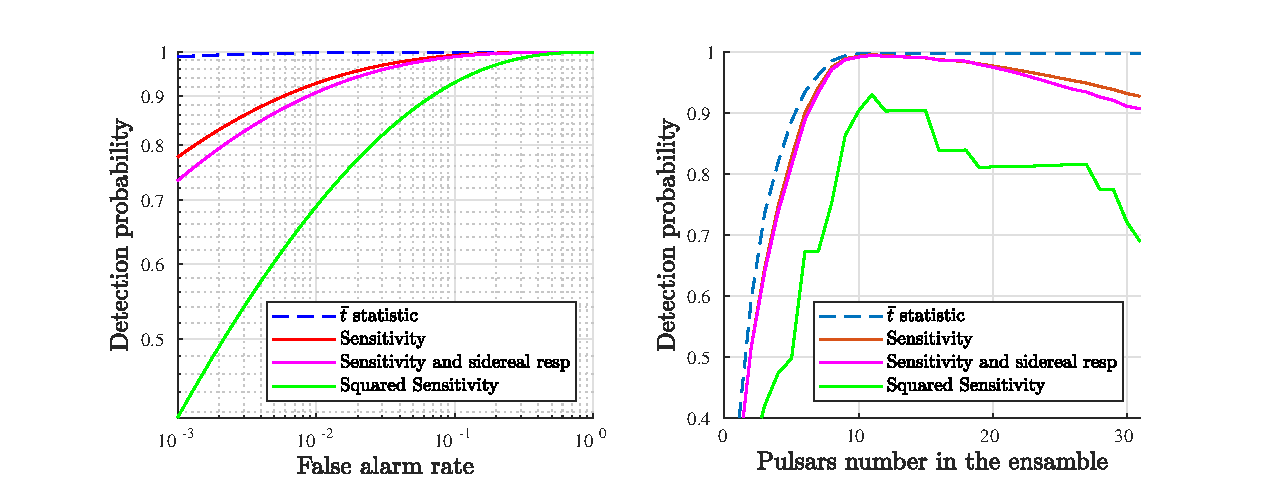
\includegraphics[clip,trim=45 0 0 10,scale=0.9]{2in1ultimo2.eps}
    \caption{On the left plot, ROC curves for the ensemble statistic for all simulated pulsars in Table \ref{realpuls} (11 pulsars with $\alpha=0.5$, 16 pulsars with $\alpha=0.1$ and 4 pulsars with $\alpha=0.04$ with injected amplitude $H=\alpha\cdot h_{min}$) and with different values of the coefficients $a_i$. On the right plot, detection probability for a false alarm rate equal to $0.01$, considering different sets of pulsars (Table \ref{realpuls}) organized for decreasing values of $\alpha$. } 
    \label{choicet}
     \vspace{-10pt}
\end{figure}
%\begin{figure}
%\centering
%\subfloat{\includegraphics[clip,trim=15 0 40 10,height=0.2\textheight, width=.45\textwidth]%{sceltat2.eps}} \quad
%\subfloat{\includegraphics[clip,trim=15 0 40 10,height=0.2\textheight, width=.45\textwidth]{PseudoROC.eps}} \\
%\caption{ROC }
%\label{fig:subfig}
%\end{figure}


\section{Scaling with number and "strength" of selected sources}\label{cinque}
Using the set of pulsar with fixed parameters in Table \ref{realpuls}, we analyzed how the detection efficiency for the ensemble depends on the number of selected pulsars and on the injected amplitudes, that is on the selected $\alpha$.
\\ First, using $\bar{t}$ statistic we checked if an analysis of ensemble could increase the detection probability in any case. Then, we evaluated the performance of the statistic with coefficients in (\ref{statt}) that could be used in real analysis.
\\Using inferred Gamma distibutions for the statistic of ensemble, we reduced computational cost avoiding software injections for each pulsar and making our analysis indipendent by O2 data. In other words, we assumed Gaussian noise for our simulations. 
\\We fix the value of $\alpha$ in (\ref{injamp}) for each pulsar considering the maximum among three possible values $\{0.04,0.1,0.5\}$ that entails injected amplitude below $50\%$ of the theoretical spin-down limit for the selected pulsar. We indicate by H4-M11-L4, for example, the ensemble of pulsar composed of 4 pulsars with "High" $\alpha=0.5$, 11 pulsars with "Medium" $\alpha=0.1$ and 4 pulsars with "Low" $\alpha=0.04$.
\begin{figure}[htpb!]
%\vspace{-30pt}
\centering
    \includegraphics[scale=0.85]{ROCbsnr.eps}
    \caption{ ROC curves for $\bar{t}$ considering different ensemble of real pulsars (Table \ref{realpuls}) with different values of $\alpha$. Adding pulsars with very low amplitude values results in minumum increase in detection efficiency. }
    \label{bnsrt}
\vspace{-10pt}    
    \end{figure}
\\As shown in Figure \ref{bnsrt} for $\bar{t}$, the detection efficiency for a chosen false alarm probability, increases considering a larger set, also if the added pulsars have "low" amplitudes. \\This happens because the coefficient $a_i$ of $\bar{t}$ is proportional to the i-th pulsar squared amplitude. In other terms, the statistic of single pulsar is weigthed by the injected amplitude.
\\In real cases, pulsars' amplitudes are unknown. For this reason, the choice in (\ref{statt}) can not take into account the effective "strength" of pulsar signal.
\\Figure \ref{appt} shows that, in this case, the increasing number of pulsars not always entails an improvement of detection efficiency. Indeed, whereas combining 4 pulsars with $\alpha=0.5$ entails an increasing of almost $50\%$ respect to the case of single pulsar, adding pulsars with lower amplitude ($\alpha=0.04,0.1$) reduces the probability of detection. 
\begin{figure}[htpb!]
\centering
    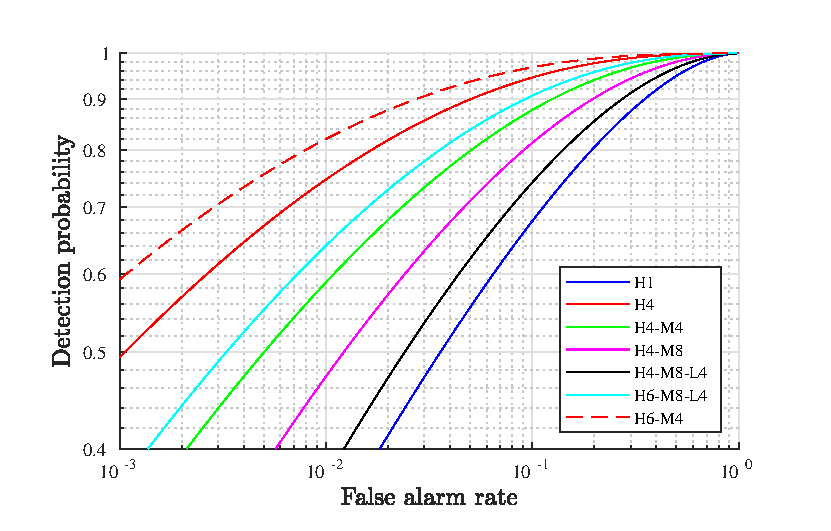
\includegraphics[scale=0.85]{ROCt.eps}
    \caption{ROC curves for the statistic $t$ with $a_i=S^{-1}(f_{gw,i})\cdot T_{obs}^{-1}$, considering different set of real pulsars (Table \ref{realpuls}) with different values of $\alpha$. In this case, adding pulsars with very low amplitude values (that is low vakues of $\alpha$) reduces the detection efficiency.  }
    \label{appt}
     \vspace{-10pt}
\end{figure}

\section{Results using O2 data} \label{6}
In this Section, we propose a new method for targeted search considering an ensemble of pulsar. We apply our method to a set of real pulsar using O2 data for Ligo detectors.
\\In principle, we can not estimate the "strength" of the expected pulsar signal since gravitational wave parameters ($\eta$, $\psi$ and $H_0$) are unknown. As described in the last Section, we need a way to organize  real pulsars in order to consider ensemble that could increase the detection efficiency. 
%\begin{wrapfloat}{figure}{o}{0pt}
%\includegraphics[clip,trim=5 0 10 10,width=0.5\textwidth]{cohe.eps}
%\caption{Noise probability density function for the coherence of single pulsar considering one detector (line in blue) and three detectors (line in red) \cite{5nvec}.}
%\label{Fig:cohe}
%\vspace{-40pt}
%\end{wrapfloat}
\\In \cite{2010}, it is introduced the coherence, defined as:
\begin{equation}\label{cohe}
c=\frac{|\hat{h}\hat{\textbf{A}}|^2}{|\textbf{X}|^2} \qquad \text{with} \qquad \textbf{A}=\hat{H}_+\textbf{A}_++\hat{H}_\times\textbf{A}_\times
\end{equation}
%where for the notation used in \cite{2010},
%\begin{equation}\label{sig}
%\textbf{A}=\hat{H}_+\textbf{A}_++\hat{H}_\times\textbf{A}_\times
%\end{equation}
and  $\hat{h}$ is the extimated \textit{complex}  amplitude, that is 
$\hat{h}=\widehat{h_0e^{i\gamma}}=\frac{\textbf{X} \cdot \textbf{A}}{|\textbf{A}|^2}$. 
\\Coherence in (\ref{cohe}) is a number between 0 and 1 that measures the resemblance between the shape of expected signal  and  data.   In  fact  it  does  not  depend  on  scaling  factors  on  the  signal  but  just on  its  shape. 
\begin{figure}[htpb!]
        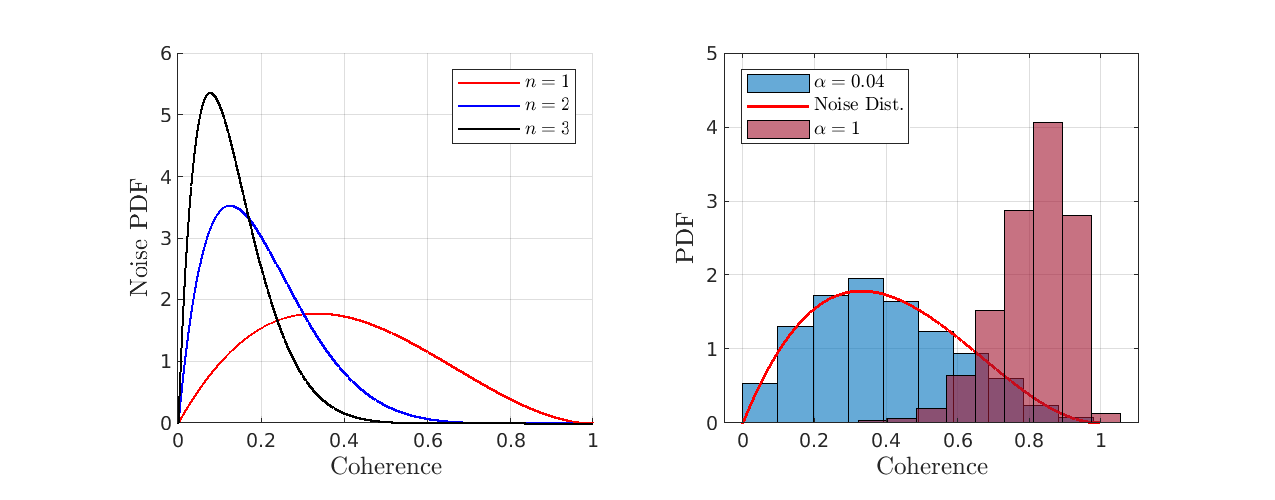
\includegraphics[clip,trim=35 0 0 10,scale=0.8]{cohe2in1.eps}
    \caption{On the left plot, theoretical noise probability distribution for coherence considering a different number $n$ of detectors, according to \cite{5nvec}. On the right plot, experimental coherence distribution for PulsarC (Table \ref{softinjABCD} and two thousand injections) considering LLO O2 run data in the frequency band $106-107$ Hz and two different $\alpha$ values ($\alpha=0.04$ in blue and $\alpha=1$ in red). For $\alpha=0.04$, experimental distribution is not distinguishable from the theoretical noise distribution. } 
    \label{pulsC}
     \vspace{-10pt}
\end{figure}
\\As showed on the left plot of Figure \ref{pulsC}, by considering more detectors (or more datasets of the same detectors) the probability of obtaining a value of coherence larger than a given threshold is a decreasing function of the number of datasets in the case of noise. In this way, by combining data from more detectors, it would be harder to get higher values of coherence with only noise.
\begin{table}[htpb!]
\begin{tabular}[t]{c|ccc}
   \multicolumn{4}{c}{\textbf{PulsarB}} \\
   \toprule
   $\alpha$ & $c_L(\alpha_L)$ &  $c_H(\alpha_H)$  & $c_{tot}$\\
\midrule 
0.04 & 0.36(0.04) & 0.52(0.03) & 0.27 \\
0.10 & 0.38(0.10) & 0.56(0.08) & 0.31 \\
0.50 & 0.58(0.48) & 0.73(0.40) & 0.56 \\
1.00 & 0.77(0.97) & 0.84(0.81) & 0.75 \\
5.00 & 0.98(4.85) & 0.98(4.04) & 0.98 \\

\bottomrule
\end{tabular}
\hspace{1cm}
\begin{tabular}[t]{c|ccc}
   \multicolumn{4}{c}{\textbf{PulsarC}} \\
\toprule
   $\alpha$ & $c_L(\alpha_L)$ &  $c_H(\alpha_H)$  & $c_{tot}$\\
\midrule 
0.04 & 0.79(0.04) & 0.17(0.03) & 0.12 \\
0.10 & 0.79(0.09) & 0.18(0.08) & 0.13 \\
0.50 & 0.86(0.48) & 0.35(0.39) & 0.35 \\
1.00 & 0.94(0.95) & 0.59(0.79) & 0.64 \\
5.00 & 0.997(4.76) & 0.96(3.97) & 0.98 \\

\bottomrule
\end{tabular}
 \caption{ Coherence values of two simulated pulsars (Table \ref{softinjABCD}) for single detector ($c_L$ for LLO and $c_H$ for LHO) and for both detectors $c_{tot}$ as a function of $\alpha$ in (\ref{injamp}) ($h_{min}$ is the minimum detectable strain considering the LLO power spectral density of 07/20/2017). $\alpha_L$ and $\alpha_H$ are computed using an avarage $h_{min}$ of all O2 run for each detector.}
\label{riscohe}
\end{table}
\\In Table \ref{riscohe}, we report the results for two simulated pulsar in Table \ref{softinjABCD} considering O2 data for Ligo detectors and different values of injected amplitudes. For LLO data, PulsarC has high coherence values also for small value of $\alpha$. This happens because coherence distributions for single detector are broad in the range $[0,1]$ for low $\alpha$ values (see right plot of Figure \ref{pulsC}). As a result, considering more detectors is important to obtain consistent values for coherence.
\\In our analysis, we used coherence as an estimation of pulsar "strength" in order to analyze ensemble of pulsars with the highest values of coherence to improve detection efficiency. Considering LLO and LHO O2 data, we organized real pulsars in Table \ref{realpuls} in decreasing values of the total coherence (see Table \ref{realpulscohe}). Since LLO O2 data are deeply no-stationary and no-Gaussian in the first months at low frequencies \cite{LLO}, we used LLO data from 04/13/2020 to the end of O2 run for pulsars with expected GW frequency below $30$ Hz. Since this procedure reduces the observation time rejecting the first three months of O2 for LLO, the sensitivity of the analysis decreses according to (\ref{hminimo}). 
\\For each pulsar, we computed  detection statistic of single pulsar for both detectors and then, we considered the weighted sum with the appropriate coefficients $a_i$ in (\ref{statt}).
\begin{figure}
\centering
        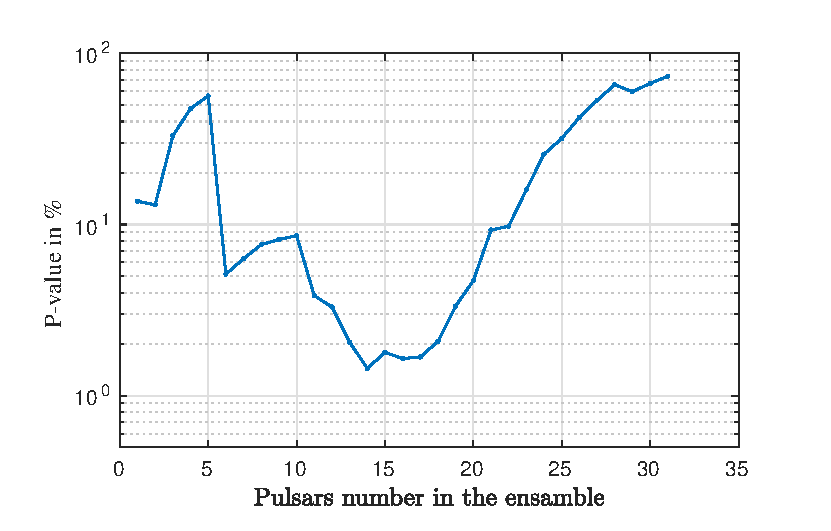
\includegraphics[clip,trim=0 0 10 0,scale=0.8]{pvalue_31.eps}
    \caption{P-values computed using the analytical noise distribution of statistic $t$ considering different sets of real pulsars (Table \ref{realpuls}) organized for decreasing values of total coherence for LLO and LHO O2 data. } 
    \label{pvalue}
     \vspace{-10pt}
\end{figure}
\\As shown in Figure (\ref{pvalue}), coherence could be a good parameter (but not optimal for O2 data) to organize real pulsars.  For instance, considering an ensemble composed of the first two pulsars and the sixth pulsar in Table \ref{realpulscohe} (see also Figure (\ref{pvalue})) the p-value is almost $0.3\%$. 
\\In any case, using analysis of ensemble, we found no evidence of CW signals in O2 data.
\section{Conclusion}\label{end}
We proposed a novel detection statistic for gravitational wave signal from an ensemble of known pulsars. The aim of this approach is to improve the detection efficiency by combining single pulsar detection based on the 5-vec method. 5-vec formalism reduces computational cost of the analysis respect to other CW pipelines. 
\\ We set theoretical limits for the coefficients $a_i$
 and using simulated pulsars to construct ROC curves, we found an approximated expression for the statistic of ensemble. This expression takes into account the detector sensitivity at the expected signal frequency of each pulsar.
%\\Figure \ref{appt} shows how the efficiency of our method depends on the strength of the injected signal. Adding weaker pulsars to the ensamble, indeed, reduces significantly the detection probability. 
\\In accordance with previous works \cite{Fstat2}, the detection efficiency increases when combining few "strong" sources and then decreases as more weaker sources are added to the ensemble. We used coherence to evaluate signal strength for real pulsar in O2 data and we found no evidence of CW signals using analysis of ensemble.
\\The described method could be applied to O3 data of LIGO detectors and also of Virgo detector using coherence to organize a larger set of real pulsars.
\\In addition, our method can be extended to a multi-detector, narrow-band search optimizing the detection statistic of ensemble. 5-vec method indeed, as described in \cite{5nvec}, can be easily extended to a network of detectors in order to improve the sensitivity of the search for single pulsar.
Moreover  5-vec method, applied to single pulsar, can be extended to narrow-band search as described in \cite{narrowband}. 
\\It is important to highlight that the detection of a gravitational wave signal of ensemble could not return information or estimations of parameters of single pulsar. However a future detection would be a clear evidence of the presence of CW signals in the analyzed data.
\clearpage
%In Ref.~\cite{ref1}...
%In Refs.~\cite{ref1,ref2}...
%On webpage~\cite{web}...

\appendix
\renewcommand{\theequation}{A.\arabic{equation}}
\section{Theoretical coefficients}\label{appendix:calcoli}
In the case of Gaussian noise with zero mean value and variance $\sigma^2$ and no signal, $S_+$ and $S_\times$ in (\ref{thstat}) have exponential distributions with mean values \cite{2014}:
\begin{equation}
\mu_{+,\times}=\frac{\sigma^2\cdot T_{obs}}{|\textbf{A}^{+,\times}|^2}=\frac{2}{k_{+,\times}} \qquad \text{with} \qquad k_{+/\times}=2 \cdot \frac{|\textbf{A}^{+/\times}|^2}{\sigma^2\cdot T_{obs}}
\end{equation} and $T_{obs}$ is the effective observation time that takes into account the detector duty cicle.
\\It follows that the mean and variance of $S$ in equation (\ref{CRS}) are:
\begin{equation}
\mu_{n}=c_+ \frac{2}{k_+} + c_\times \frac{2}{k_\times} \qquad \Theta_{n}^{\,2}=c_+^{\,2} \frac{4}{k_+^{\,2}} + c_\times^{\,2} \frac{4}{k_\times^{\,2}}
\end{equation}
If a signal is present into data, $S_+$ and $S_\times$ have non central $\chi^2$ distributions (unless the factor $k_{+/\times}$) with two degrees of freedom. Altough there is no simple expression for the distribution of $S$, the mean value in this case is:
\begin{equation}
\mu_{sig}=c_+ \frac{2+\beta_+}{k_+} + c_\times \frac{2+\beta_\times}{k_\times}
\end{equation}where\begin{equation}
\beta_{+/\times}=2\frac{H_0^2|e^{j\Phi_0}H_{+/\times}\textbf{A}^{+/\times}|^2}{\sigma^2\cdot T_{obs}}=H_0^2|H_{+/\times}|^2k_{+/\times}
\end{equation}
The critical ratio ($\textrm{CR}$) for the statistic of single pulsar is:
\begin{equation}
 \textrm{CR}= \frac{\left( c_+ \frac{\beta_+}{k_+} + c_\times \frac{\beta_\times}{k_\times}\right)^2}{\left(c_+^{\,2} \frac{4}{k_+^{\,2}} + c_\times^{\,2} \frac{4}{k_\times^{\,2}}\right)} 
\end{equation}
We need to solve the following system to maximize the $\textrm{CR}$:
\begin{equation}
\left\{ \begin{array}{lr} \frac{\partial (\textrm{CR})}{\partial c_+} = 2\frac{\beta_+}{k_+}(c_+^{\,2}\frac{4}{k_+^{\,2}}+c_\times^{\,2}\frac{4}{k_\times^{\,2}})-2c_+\frac{4}{k_+^{\,2}}(c_+\frac{\beta_+}{k_+}+c_\times\frac{\beta_\times}{k_\times}) =0   \vspace*{0.3cm}\\ \frac{\partial (\textrm{CR})}{\partial c_\times} = 2\frac{\beta_\times}{k_\times}(c_+^{\,2}\frac{4}{k_+^{\,2}}+c_\times^{\,2}\frac{4}{k_\times^{\,2}})-2c_\times\frac{4}{k_\times^{\,2}}(c_+\frac{\beta_+}{k_+}+c_\times\frac{\beta_\times}{k_\times}) = 0 \end{array}\right. 
\end{equation}
The two equations are not independent. There is a straight line in the plane $(c_+,c_\times)$ where the function $\textrm{CR}$ has maximum value. This line is identified by the equation:
\begin{equation}\label{der}
c_+=\beta_+k_+\frac{c_\times}{\beta_\times k_\times}=|H_+|^2|\textbf{A}_+|^4\frac{c_\times}{|H_\times|^2|\textbf{A}_\times|^4}
\end{equation}
In this case, you can chose arbitrarily that:
\begin{equation}\label{chos}
\bar{c}_+=|H_+|^2|\textbf{A}_+|^4 \qquad \text{and} \qquad \bar{c}_\times=|H_\times|^2|\textbf{A}_\times|^4
\end{equation}
In the same way, it is possible to infer the best $\textrm{CR}$ choice for the coefficients $a_i$ of the statistic of ensamble $t$, defined as:
\begin{equation}
t=\sum_{i=1}^{N_s} a_i S_i
\end{equation}where $N_s$ is the number of pulsars and $S_i$ is the statistic of single pulsar defined as:
\begin{equation}
S_i=b_{+,i}S_{+,i} + b_{\times,i}S_{\times,i} \qquad \text{with} \qquad b_{+,i}\equiv c_+ \qquad b_{\times,i}\equiv c_\times
\end{equation}
In this case, the critical ratio is:
\begin{equation}
\textrm{CR}= \frac{\left[\sum_{j=1}^{N_s} a_j \left( b_{+,j} \frac{\beta_{+,j}}{k_{+,j}} + b_{\times,j} \frac{\beta_{\times,j}}{k_{\times,j}}\right)\right]^2}{\sum_{i=1}^{N_s} a_i^2 \left(b_{+,i}^{\,2} \frac{4}{k_{+,i}^{\,2}} + b_{\times,i}^{\,2} \frac{4}{k_{\times,i}^{\,2}}\right)} = \frac{\left[\sum_{j=1}^{N_s} a_j \lambda_j\right]^2}{\sum_{i=1}^{N_s} a_i^2 \Sigma_i^{\,2}}
\end{equation}
\begin{equation}
\hspace*{-2.5cm} \text{with} \qquad \lambda_j\equiv b_{+,j} \frac{\beta_{+,j}}{k_{+,j}} + b_{\times,j} \frac{\beta_{\times,j}}{k_{\times,j}} \qquad \text{and} \qquad \Sigma_j^{\,2}\equiv b_{+,j}^{\,2} \frac{4}{k_{+,j}^{\,2}} + b_{\times,j}^{\,2} \frac{4}{k_{\times,j}^{\,2}}
\end{equation}
Maximizing the $\textrm{CR}$ for the coefficients $a_k$, we found:
\begin{equation}
\frac{\partial (\textrm{CR})}{\partial a_k}=\frac{2\lambda_k\left(\sum_{j=1}^{N_s}a_j \lambda_j\right)}{\sum_{i=1}^{N_s}a_i^2\Sigma^2_i}-\frac{2a_k \Sigma_k^2\left(\sum_{j=1}^{N_s}a_j \lambda_j\right)^2}{\left(\sum_{i=1}^{N_s}a_i^2\Sigma^2_i\right)^2}=0
\end{equation}
%\begin{equation}
%\lambda_k \left(\sum_{i=1}^{N_s}a_i^2\sigma^2_i\right) - a_k \sigma_k^2\left(\sum_{j=1}^{N_s}a_j \lambda_j\right)=0
%\end{equation}
As in the case of single pulsar, there is an hyperplane where the function $\textrm{CR}(a_1,..,a_{N_s})$ has the maximum value,
\begin{equation}
a_k=\frac{\lambda_k}{\Sigma_k^2}\frac{\left(\sum_{i=1,i\neq k}^{N_s}a_i^2\Sigma^2_i\right)}{\left(\sum_{j=1,j\neq k}^{N_s}a_j \lambda_j\right)}
\end{equation}and a particular, simple choice is:
\begin{equation}
\bar{a}_k=\frac{\lambda_k}{\Sigma_k^{\,2}}=\frac{H_{0,k}^2}{\sigma^4_k\cdot T_{obs}^2 } 
\end{equation}



\clearpage
\section{Pulsars parameters}
\begin{table}[h!]
%\setlength{\tabcolsep}{5pt}
%\renewcommand{\arraystretch}{1.5}
  \begin{center}
  	\begin{tabular}{c| c c c c c c}
  	\toprule
  \textbf{Inj. name} & $(a,\delta)$ & $f_0$ $[Hz]$ & $\dot{f}_0$ $[Hz/s]$ & $\alpha$  & $\eta$ & $\psi$  \\
      \midrule
     PulsarA & (178.37,-33.43) & 106.71 &  0 & 0.50 & 0.28 & 42 \\
     PulsarB & (150.33,-10.76) & 106.24 & 7 $\cdot$ 10$^{-11}$ & 0.50 & 0.44 & 22 \\
     PulsarC & (120.32,10.45) & 106.57 & 7 $\cdot$ 10$^{-18}$ & 0.70 & 0.16 & 28 \\
     PulsarD & (90.33,30.76) & 106.83 & 7 $\cdot$ 10$^{-11}$ & 0.70 & 0.13 & 27\\
      \bottomrule
   		 \end{tabular}
  \end{center}
  \caption{ Table of the software injected signals parameters, used to evaluate the noise and signals distributions of $t$. The position of these "injected" sources is specified by the right ascension $a$ and by the declination $\delta$ in degrees. The injected amplitude $H$ is equal to $H=\alpha\cdot h_{min}$ with $0<\alpha<1$. }
  \label{softinjABCD}
\end{table}



\begin{table}[h!]\hspace{-0.8cm}
\begin{tabular}[t]{c|ccc}
\toprule
   \textbf{Pulsar name} & $f_{gw}$ $[Hz]$ &  $h_ {sd}$  & $\alpha$\\
\midrule 
J0030-0451  & 411.06 & 3.90 $\cdot$ 10$^{-27}$ & 0.04 \\
J0437-4715 & 347.38 & 1.60 $\cdot$ 10$^{-26}$ & 0.10 \\
J0534-2200 & 59.33  & 5.00 $\cdot$ 10$^{-26}$  & 0.50 \\
J0835-4510 & 22.39  & 2.90 $\cdot$ 10$^{-25}$ & 0.50 \\
J0940-5428 & 22.84  & 1.20 $\cdot$ 10$^{-25}$ & 0.10 \\
J1028-5819 & 21.88  & 1.20 $\cdot$ 10$^{-25}$ & 0.10 \\
J1105-6107 & 31.65  & 6.00 $\cdot$ 10$^{-26}$ & 0.50 \\
J1112-6103 & 30.78  & 1.90 $\cdot$ 10$^{-26}$ & 0.10 \\
J1300-1240 & 321.62 & 5.80 $\cdot$ 10$^{-27 }$ & 0.10 \\
J1420-6048 & 29.64  & 1.60 $\cdot$ 10$^{-25}$ & 0.50 \\
J1509-5850 & 22.49  & 6.70 $\cdot$ 10$^{-26}$ & 0.10 \\
J1531-5610 & 23.75  & 1.10 $\cdot$ 10$^{-25}$ & 0.10 \\
J1537-1155 & 52.76  & 6.10 $\cdot$ 10$^{-27 }$ & 0.10 \\
J1809-1917 & 24.17  & 1.40 $\cdot$ 10$^{-25}$ & 0.50 \\
J1809-2332 & 13.62  & 4.43 $\cdot$ 10$^{-25}$ & 0.04 \\
J1813-1246 & 41.60  & 1.90 $\cdot$ 10$^{-25}$ & 0.50 \\
\midrule
\end{tabular}
\hspace{0.5cm}
\begin{tabular}[t]{c|ccc}
\toprule
  \textbf{Pulsar name} & $f_{gw}$ $[Hz]$ &  $h_ {sd}$  & $\alpha$\\
\midrule 
J1826-1256 & 18.14  & 6.92 $\cdot$ 10$^{-25}$ & 0.50 \\
J1828-1101 & 27.75  & 5.00 $\cdot$ 10$^{-26}$ & 0.10 \\
J1831-0952 & 29.73  & 7.70 $\cdot$ 10$^{-26}$ & 0.50 \\
J1833-0827 & 23.45  & 6.20 $\cdot$ 10$^{-26}$ & 0.10 \\
J1837-0604 & 20.77  & 8.90 $\cdot$ 10$^{-26}$ & 0.10 \\
J1841-0130 & 67.18  & 4.20 $\cdot$ 10$^{-27 }$ & 0.04 \\
J1856-0245 & 24.72  & 6.90 $\cdot$ 10$^{-26}$& 0.10 \\
J1913-1011 & 55.70  & 5.40 $\cdot$ 10$^{-26}$& 0.50 \\
J1925-1720 & 26.43  & 3.10 $\cdot$ 10$^{-26}$& 0.10 \\
J1928-1746 & 29.10  & 4.33 $\cdot$ 10$^{-26}$& 0.10 \\
J1935-2025 & 24.96  & 8.10 $\cdot$ 10$^{-26}$& 0.10 \\
J1952-3252 & 50.59  & 1.00 $\cdot$ 10$^{-25}$& 0.50 \\
J2043-2740 & 20.80  & 6.30 $\cdot$ 10$^{-26}$ & 0.10 \\
J2124-3358 & 405.59 & 4.10 $\cdot$ 10$^{-27}$ & 0.04 \\
J2229-6114 & 38.71  & 3.30 $\cdot$ 10$^{-25}$ & 0.50\\
\bottomrule
\end{tabular}
 \caption{ Table of the real pulsars used in this work. $h_{sd}$ is the spin-down amplitude \cite{JKS,narrowband}. Source parameters (position, distance, frequency and frequency evolution) are taken from the Australia Telescope National Facility (ATNF) Pulsar Catalogue \cite{atnf}. The injected amplitude $H$, equal to $H=\alpha\cdot h_{min}$ with $0<\alpha<1$, satisfies the condition $H< 0.50\cdot h_{sd}$. }
\label{realpuls}
\end{table}
\clearpage

\section{Coherence values for O2 data}
\begin{center}
\begin{table}[h!]
\begin{tabular}[t]{c|ccc}
\toprule
   \textbf{Pulsar name} & $c_L$ &  $c_H$  & $c_{tot}$ \\
\midrule 
J1028-5819 & 0.468 & 0.797 & 0.609 \\
J1826-1256 & 0.213 & 0.844 & 0.592 \\
J1531-5610 & 0.785 & 0.581 & 0.483 \\
J1828-1101 & 0.296 & 0.517 & 0.399 \\
J1420-6048 & 0.31  & 0.605 & 0.385 \\
J1300-1240 & 0.779 & 0.412 & 0.379 \\
J1112-6103 & 0.073 & 0.554 & 0.376 \\
J1837-0604 & 0.306 & 0.567 & 0.332 \\
J1952-3252 & 0.755 & 0.431 & 0.33  \\
J1925-1720 & 0.358 & 0.349 & 0.313 \\
J1935-2025 & 0.343 & 0.516 & 0.276 \\
J2229-6114 & 0.638 & 0.249 & 0.275 \\
J1813-1246 & 0.729 & 0.352 & 0.274 \\
J2043-2740 & 0.89  & 0.297 & 0.266 \\
J1833-0827 & 0.222 & 0.516 & 0.254 \\
J0940-5428 & 0.464 & 0.375 & 0.208 \\
\midrule
\end{tabular}
\hspace{0.5cm}
\begin{tabular}[t]{c|ccc}
\toprule
  \textbf{Pulsar name} & $c_L$ &  $c_H$  & $c_{tot}$\\
\midrule 
J1831-0952 & 0.631 & 0.211 & 0.178 \\
J1809-2332 & 0.557 & 0.691 & 0.178 \\
J1509-5850 & 0.166 & 0.182 & 0.157 \\
J1913-1011 & 0.503 & 0.455 & 0.149 \\
J0534-2200 & 0.261 & 0.512 & 0.129 \\
J0835-4510 & 0.481 & 0.079 & 0.117 \\
J1105-6107 & 0.421 & 0.083 & 0.113 \\
J1537-1155 & 0.085 & 0.314 & 0.109 \\
J1809-1917 & 0.206 & 0.221 & 0.108 \\
J2124-3358 & 0.28  & 0.023 & 0.096 \\
J1841-0130 & 0.181 & 0.047 & 0.083 \\
J0437-4715 & 0.268 & 0.071 & 0.076 \\
J0030-0451  & 0.444 & 0.729 & 0.058 \\
J1928-1746 & 0.375 & 0.138 & 0.033 \\
J1856-0245 & 0.196 & 0.02  & 0.014 \\
\bottomrule
\end{tabular}
 \caption{ Coherence values of real pulsars (Table \ref{realpuls}) for single detector ($c_L$ for LLO and $c_H$ for LHO) and for both detectors $c_{tot}$. For pulsars with expected GW frequency below $30$ Hz,  we used LLO data from 04/13/2020 to the end of O2 run.}
\label{realpulscohe}
\end{table}
\end{center}

\clearpage
\section*{References}
\begin{thebibliography}{10}

\bibitem{firstdet}  LIGO Scientific Collaboration and Virgo Collaboration, \emph{Observation of Gravitational Waves from a Binary Black Hole Merger}, Physical Review Letter 116,061102 (2016)
 
\bibitem{astimpl} LIGO Scientific Collaboration and Virgo Collaboration ,\emph{Astrophysical implications of the binary black hole merger GW150914}, The Astrophysical Journal Letters, 818:L22 (2016) 

\bibitem{firstBBS} LIGO Scientific Collaboration and Virgo Collaboration, \emph{GW170817: Observation of Gravitational Waves from a Binary Neutron Star Inspiral}, Physical Review Letter 119,161101 (2017)

\bibitem{result} LIGO Scientific Collaboration and Virgo Collaboration, \emph{Searches for Gravitational Waves from Known Pulsars at Two Harmonics in 2015–2017 LIGO Data}, LIGO-P1800344 (2019)

\bibitem{Fstat2}Y. Chen ,C. Messenger, X. Fan, \emph{Method to detect gravitational waves from an ensemble of known pulsars}, Phys. Rev. D 94 (2016)

\bibitem{bayes}  M. Pitkin, C. Messenger, X. Fan, \emph{Hierarchical Bayesian method for detecting continuous gravitational waves from an ensemble of pulsars}, Phys. Rev. D 98, 063001 (2018)

\bibitem{2010} P. Astone et al., \emph{A method for detection of known sources of continuous gravitational wave signals in non-stationary data}, Class. Quantum Grav. 27 (2010) 

\bibitem{2019} O. J. Piccinni et al., \emph{A new data analysis framework for the search of continuous gravitational wave signals}, Class. Quantum Grav. 36 (2019)

\bibitem{JKS} P. Jaranowski, A. Kròlak and B. F. Schutz \emph{Data analysis of gravitational wave signals from spinning neutron stars}, Phys. Rev. D,58(6):063001 (1998)

\bibitem{2014} P. Astone et al., \emph{Method for narrow-band search of continuous gravitational wave signals}, Phys. Rev. Lett. 062008 (2014)

\bibitem{jjj}Leaci, P. and the LIGO Scientific Collaboration and the Virgo Collaboration, \emph{Searching for continuous gravitational wave signals using
LIGO and Virgo detectors}, J. Phys.: Conf. Ser. 354 012010 (2012).

\bibitem{atnf} ATNF Pulsar Catalogue, Catalogue Version 1.61, https://www.atnf.csiro.au/research/pulsar/psrcat/

\bibitem{LLO}  aLIGO LLO Logbook, \emph{ER10 vs O2 calibration lines and noise floor}, Monday 03 April 2017 (32763), https://alog.ligo-la.caltech.edu/aLOG/index.php?callRep=32763

\bibitem{5nvec} P. Astone et al., \emph{Coherent search of continuous gravitational wavesignals: extension of the 5-vectors method to anetwork of detectors},  Journal of Physics: Conference Series, Volume 363 (2012)

\bibitem{narrowband}LIGO Scientific Collaboration and Virgo Collaboration, \emph{Narrow-band search for gravitational waves from known pulsars using the second LIGO observing run}, Phys. Rev. D 99, 122002 (2019)


%\bibitem{ref1} J.~Doe, Article name, \textit{Phys. Rev. Lett.}

%\bibitem{ref2} J.~Doe, J. Smith, Other article name, \textit{Phys. Rev. Lett.}

%\bibitem{web} \href{http://www.google.pl}{www.google.pl}

\end{thebibliography}

\end{document}

